\section{Synthesis objectives and chosen approach\label{section:inductive-objectives-and-approach}}

This section gives an overview of the synthesis approach. Section~\ref{subsection:inductive-synthesis-statement} states the problem statement in terms of the formal models of Chapter~\ref{chapter:framework}. Section~\ref{subsection:inductive-synthesis-requirements} completes this by stating additional requirements on the synthesis approach. Section~\ref{subsection:inductive-synthesis-approach} presents an overview of our inductive-oriented approach, in the light of those requirements.

%%%

\subsection{Problem statement\label{subsection:inductive-synthesis-statement}}

In its simplest form, the problem of synthesizing LTS state machines from MSC scenarios can be stated as follows:

\begin{quotation}
\noindent \underline{Given}~~a consistent scenario collection showing typical examples and counterexamples of system behaviors

\vspace{-0.7cm}
\begin{align*}
Sc = (S^+,S^-)
\end{align*}

\vspace{-0.2cm}
\noindent \underline{Synthesize}~~the system as a composition of agent LTSs

\vspace{-0.7cm}
\begin{align*}
System = (Ag_1 \parallel \ldots \parallel Ag_n)
\end{align*}

\vspace{-0.2cm}
\noindent \underline{Such that}~~$Sc$ and $System$ are consistent.
\end{quotation}

\noindent For recall, the consistency condition covers three criteria (see Section~\ref{subsection:background-scenario-consistency}):

\begin{itemize}
\item \textbf{structural consistency} -- the state machine and scenario views are \emph{structurally} consistent, that is, they agree on the agent decomposition and their respective interface,
\item \textbf{consistent agent view} -- the timelines of any positive scenario $P \in S^+$ specify existing paths in the corresponding agent state machines. The same applies for the precondition of any negative scenario $N \in S^-$.
\item \textbf{consistent system view} -- the system correctly accepts positive scenarios and preconditions of negatives ones. It also correctly rejects negative scenarios. We recall below the precise conditions from Section~\ref{subsection:background-scenario-consistency}:
\begin{align*}
\mathcal{L}(System) &= \mathcal{L}^+(Sc)\\
\mathcal{L}(System) \cap \mathcal{L}^-(Sc) &= \emptyset
\end{align*}

\end{itemize}

%%%

\subsection{Synthesis requirements\label{subsection:inductive-synthesis-requirements}}

The characterization above provides a precise statement in terms of the formal models of Chapter~\ref{chapter:framework}. This statement is completed with a few usability requirements.

\noindent \textbf{Flexibility} -- keeping a flexible approach with respect to the input scenario language looks important for end-user involvement and usability:
\begin{itemize}

\item End-users are most likely to be unable to provide rich scenario descriptions in the early phases of system design. This includes state assertions along scenario episodes or flowcharts on such episodes. The synthesis approach should be usable when only a few scenarios are available.

\item Both positive and negative scenarios should be taken into account. Negative scenarios are not uncommon among the examples provided by stakeholders. One reason is that they naturally illustrate violations of safety goals while being easier to specify than the latter. 

\item System analysis is incremental by nature. Richer input scenarios are therefore very likely to be \emph{eventually} available. The synthesis approach should help incrementally refining a first scenario specification towards richer models. It should also gracefully adapt to work on such richer input in advanced analysis phases.

\end{itemize}

\noindent \textbf{Behavior generalization} -- the synthesis approach must at least cover the behaviors described in the positive scenarios. In most cases, scenarios provide \emph{examples} of system behaviors and are inherently incomplete. Synthesized state machines should therefore cover more behaviors than those already described. 

An upper bound on behavior generalization is given by the consistency condition, that requires negative scenarios to be correctly rejected. This upper bound has to be refined when other models are available (see below).

\noindent \textbf{Multi-model consistency} -- the possibility of having richer input models suggests taking other models into account, such as fluents or goals, in addition to scenarios. These models should not be \emph{required} as input, but are better \emph{supported} when available. 

In such case, our characterization must be strengthened. In input, all available models shall be required to be consistent with each other. In output, the synthesized system shall be consistent with all models. Notably, the synthesized system should not violate known safety goals.

%%%

\subsection{Approach overview\label{subsection:inductive-synthesis-approach}}

Figure~\ref{image:inductive-synthesis-overview} shows the two main steps of our synthesis approach for the simple case where only a scenario collection is taken as input. 

\begin{figure}[H]\centering
  \scalebox{0.55}{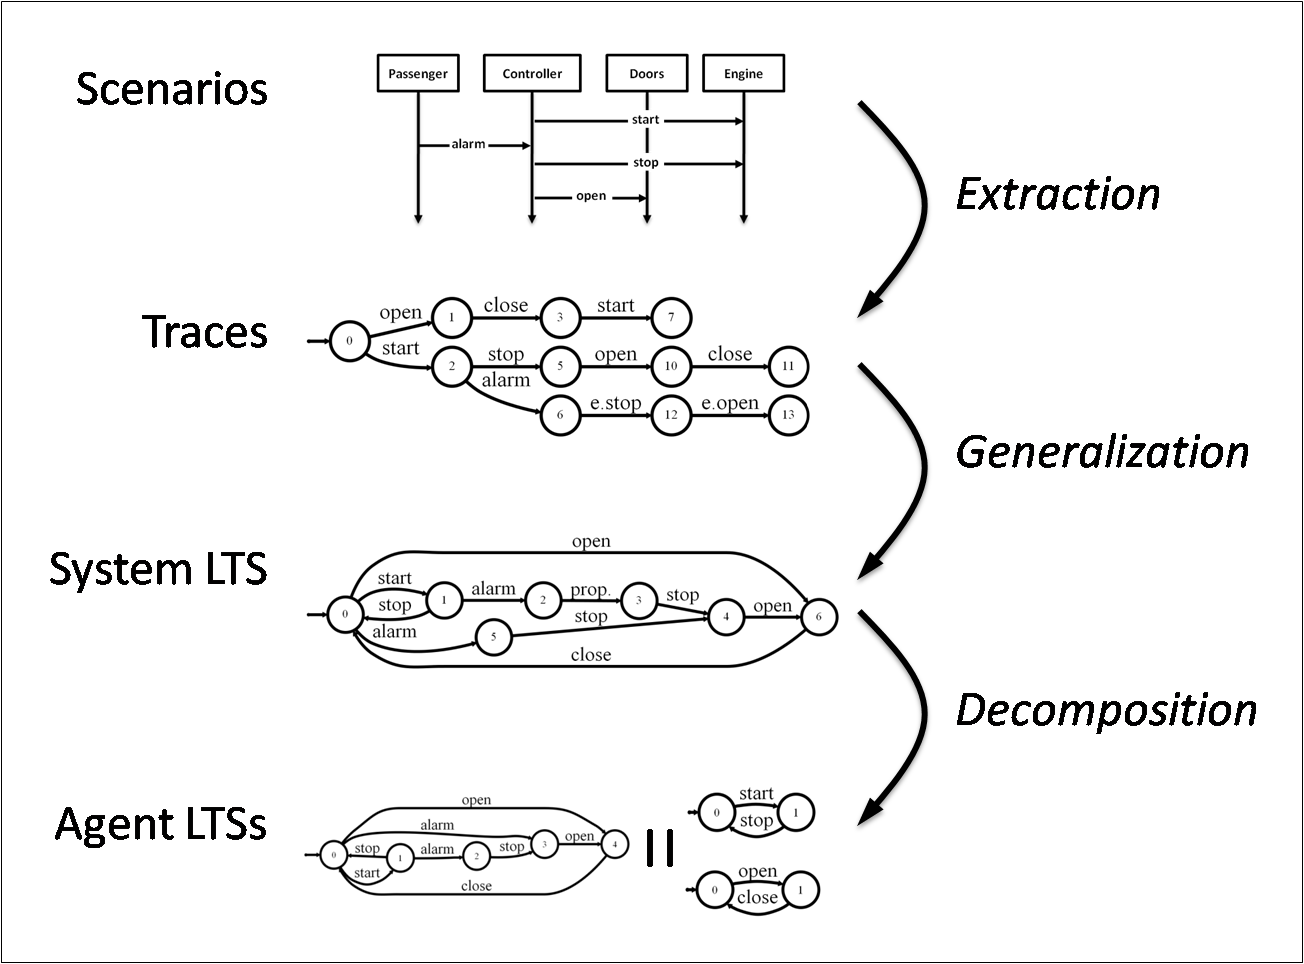
\includegraphics[trim=3mm 3mm 10mm 3mm, clip]{src/4-inductive/images/overview}}
  \caption{Overview of inductive LTS synthesis from MSCs.\label{image:inductive-synthesis-overview}}
\end{figure}

The \underline{generalization} step extends grammar induction techniques developed in \cite{Oncina:1992} to synthesize a System LTS covering all positive scenarios and excluding all negative ones. The generalization strategy is borrowed from the Regular Positive and Negative Inference (RPNI) algorithm~\cite{Oncina:1992} and proceeds as follows.

An initial automaton $A_0$ accepting exactly the positive traces is incrementally refined by merging well chosen state pairs.
Doing so generalizes accepted behaviors; this process is performed under the control of the negative scenarios to avoid over-generalization. Every intermediate solution $A_i$ respects the \emph{consistent system view}; the latter therefore provides a useful algorithm invariant:
\begin{align*}
\mathcal{L}(A_i) &\subseteq \mathcal{L}^+(Sc)\\
\mathcal{L}(A_i) \cap \mathcal{L}^-(Sc) &= \emptyset
\end{align*}

The \underline{decomposition} step computes a LTS for each agent by projecting the System LTS on their respective alphabet. It makes use of standard hiding, determinization and minimization operators on automata \cite{Hopcroft:1979}. 

For an agent $Ag$ the projection of the System LTS $S$ is given by:
\begin{align}
(S \setminus \Sigma_{Ag}^c)^\Delta
\end{align}
\noindent where $\Sigma_{Ag}^c$ denotes the set of all system events but those of $Ag$'s interface.

\subsubsection*{A word about correctness}

The decomposition step ensures that the \emph{structural consistency} and \emph{consistent agent view} conditions hold. It is a straightforward application of the material given in Chapter~\ref{chapter:framework}. 

The generalization invariant guarantees that the \emph{consistent system view} condition holds for the System LTS. The approach is correct only if the same condition holds for the system re-composition $\system$. This might not be the case in presence of negative implied scenarios. This issue is further examined in Section~\ref{section:inductive-discussion}.

\subsubsection*{Integration of additional requirements}

The RPNI-driven generalization step provides a first milestone towards an inductive LTS synthesis approach that meets our requirements. It generalizes scenario collections without requiring additional state or flowchart information. However, such approach does not provide much flexibility; multi-model consistency is not guaranteed either. Section \ref{section:inductive-background} covers this first milestone through background on grammar induction and RPNI.

Section~\ref{section:lts-induction-from-mscs} introduces our Query-driven State Merging (QSM) algorithm that extends RPNI with an interactive feature. The latter supports the elicitation of additional, ``interesting'' scenarios that are not originally provided by the end-user. The original collection of scenarios is completed by asking the user scenario queries that are generated during synthesis. A \emph{scenario query} consists of showing the user a specific scenario and asking her to classify it as positive or negative. This guides the generalization process towards more accurate state machines while enriching input scenario models.

The multi-view consistency requirement is tackled in Section~\ref{section:inductive-mutliview-consistency}. QSM is extended so as to allow the injection of additional information that constrain the induction and prune the inductive search space. Additional information may include global definitions of fluents; declarative properties of the domain; behavior models of external components; and goals that the software system is expected to satisfy. Doing so guarantees the consistency of synthesized state machines with all other models.

Managing the consistency of a large scenario collection is challenging; hMSCs partly address this through a structured form of scenarios that allows reuse. Section~\ref{section:inductive-from-hMSC} shows how hMSCs can replace scenario collections as input of the generalization process. In this setting, negative scenarios and other models can still be used to constraint the inductive search space and guarantee consistency. At the time of writing, however, the interactive feature of QSM is a work in progress.

Taking hMSCs as input implies both a theoretical and practical shift of perspective. It leads us considering the generalization of state machines under the control of safety goals as a natural extension of the generalization of positive scenarios under the control of negative ones. Among others, this question is further discussed in Section~\ref{section:inductive-discussion}.
